\documentclass{article}
\usepackage{tikz}
\usepackage[simplified]{pgf-umlcd}
\usepackage{multirow}
\usepackage{float}
\usetikzlibrary{arrows, arrows.meta}

\begin{document}

\title{
    Tarea 1 - Modelo y Diccionario \\
    INF239 - BASES DE DATOS
}
\author{
    Matías Peñaloza 202373037-8 \\
    Hans González 202373020-3
}
\date{
    2025-1
}
\maketitle

\section{Modelo}
Se presenta a continuación el modelo de la base de datos:
\begin{center}
\resizebox{1.1\textwidth}{!}{
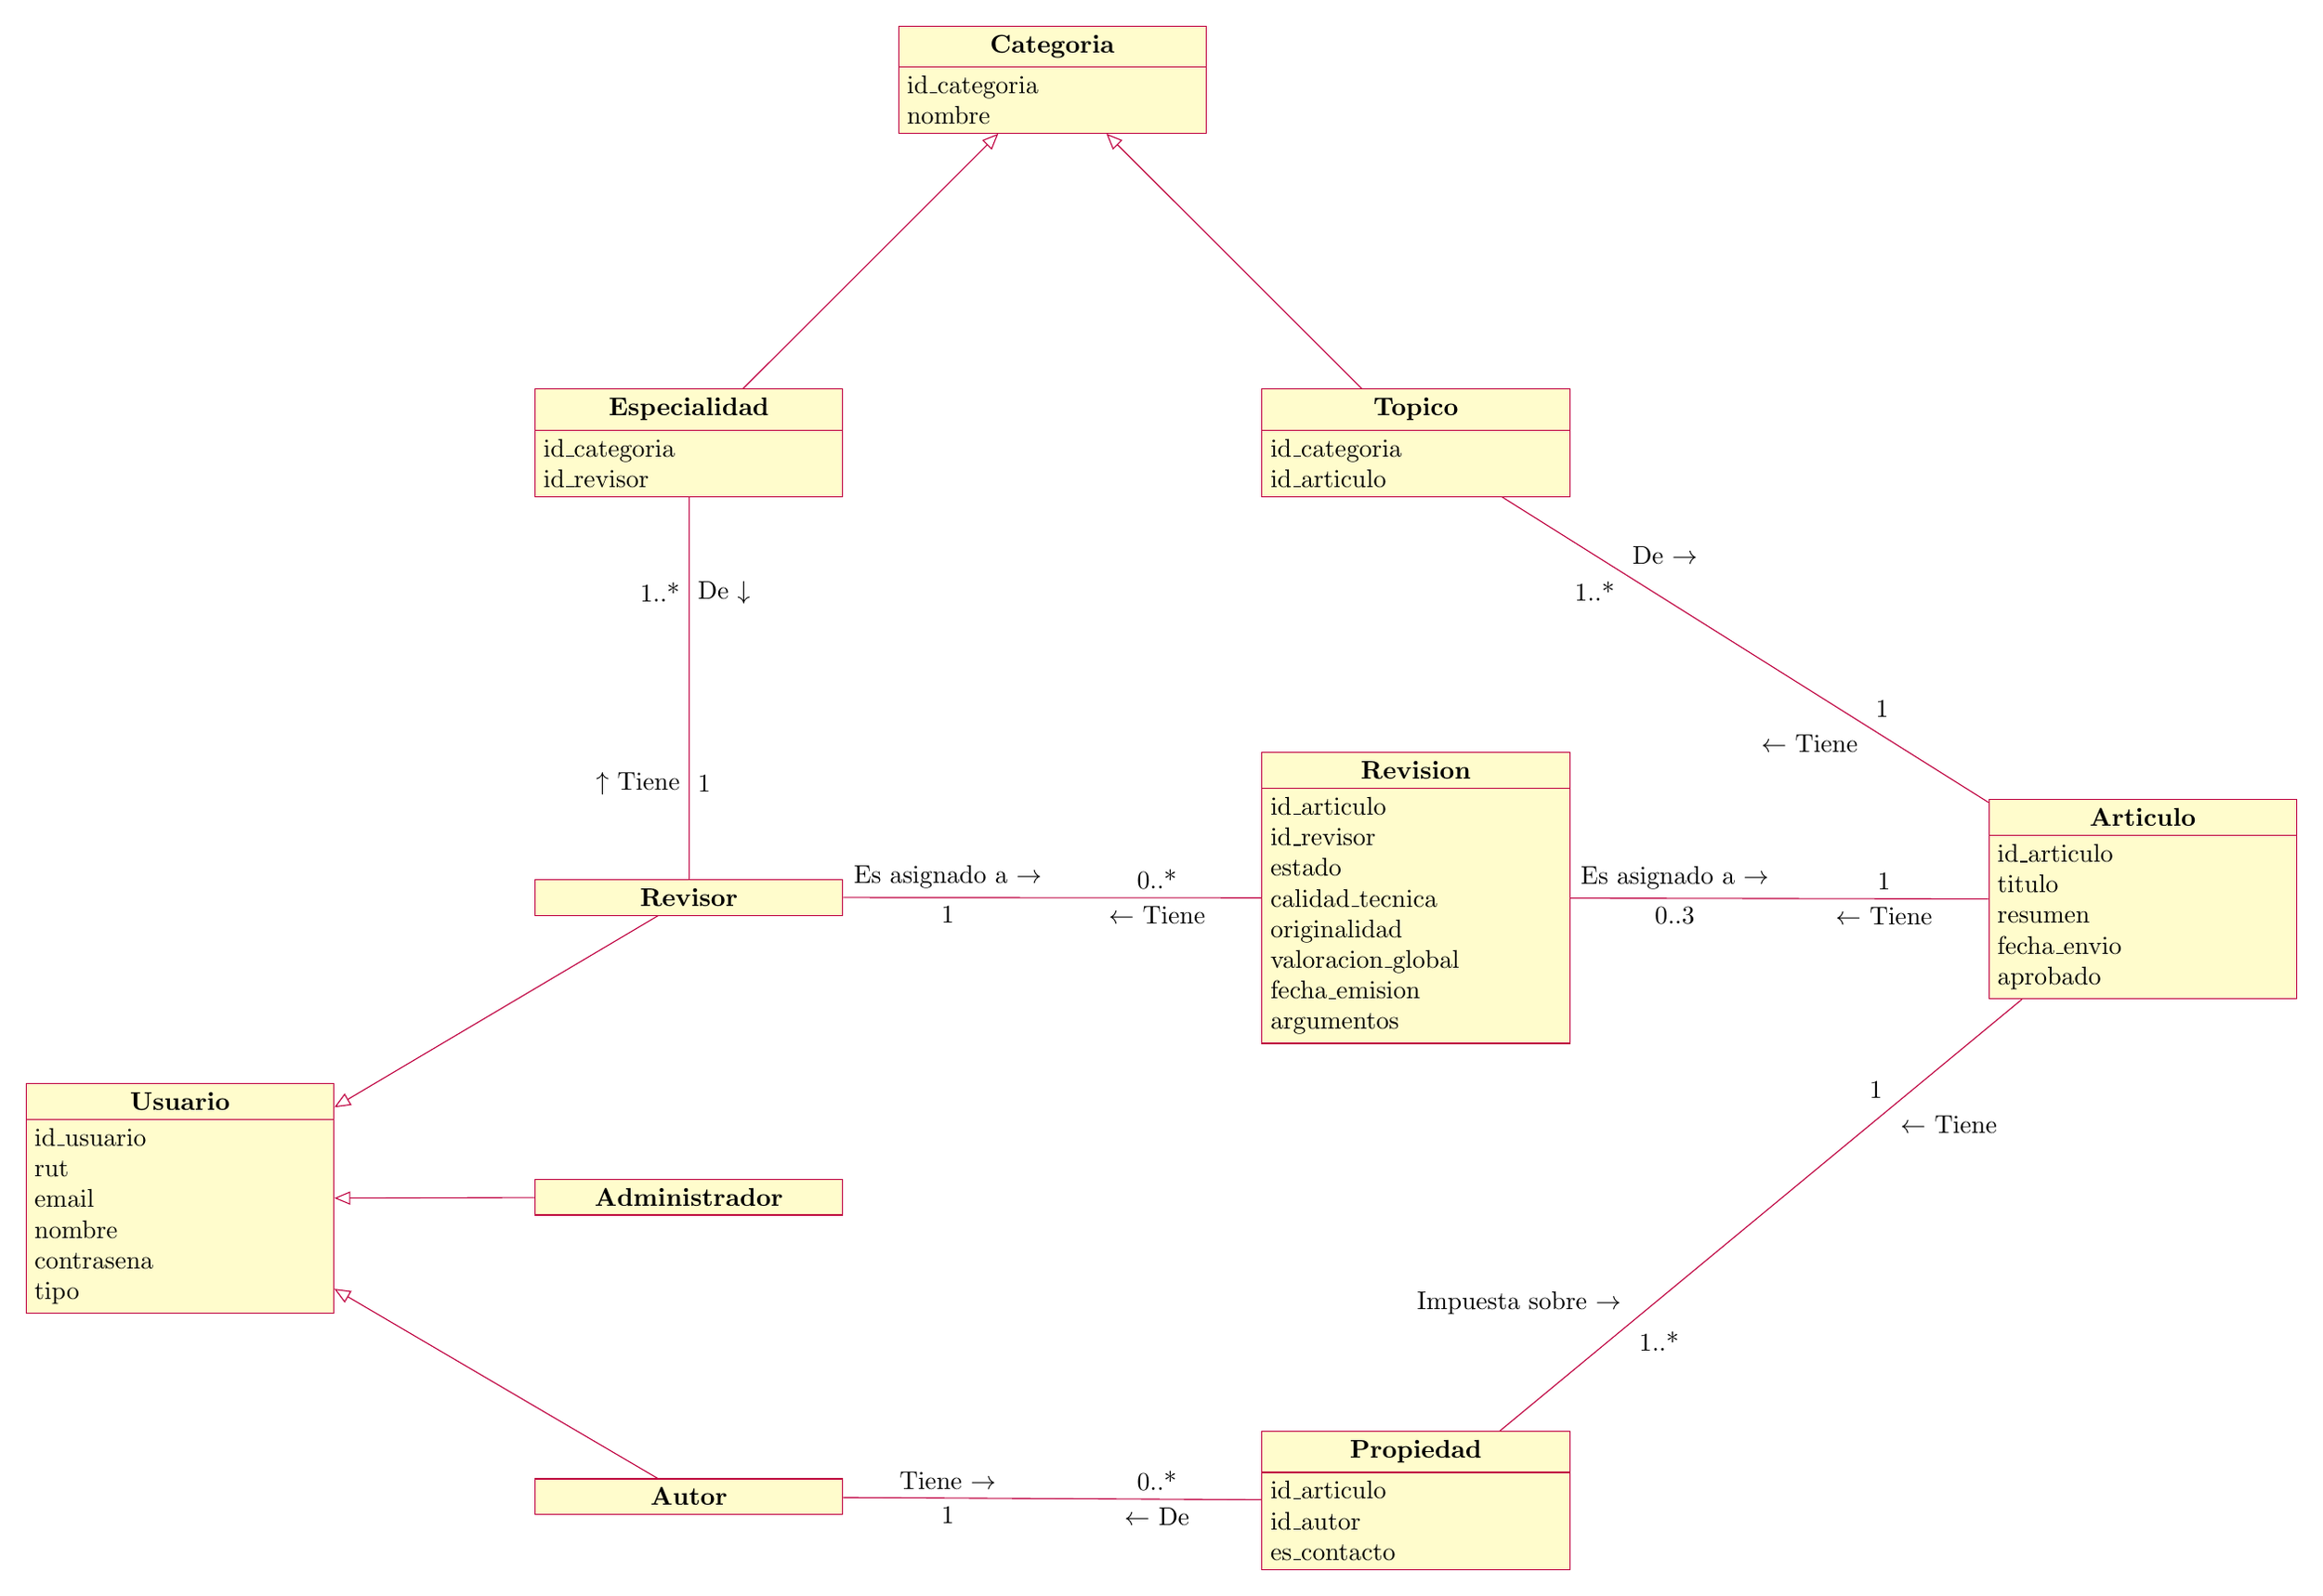
\begin{tikzpicture}

\begin{class}[text width=4cm]{Categoria}{0, 0}
    \attribute{id\_categoria}
    \attribute{nombre}
\end{class}

\begin{class}[text width=4cm]{Topico}{5, -5}
    \inherit{Categoria}
    \attribute{id\_categoria}
    \attribute{id\_articulo}
\end{class}

\begin{class}[text width=4cm]{Especialidad}{-5, -5}
    \inherit{Categoria}
    \attribute{id\_categoria}
    \attribute{id\_revisor}
\end{class}

\begin{class}[text width=4cm]{Usuario}{-12, -14.56}
    \attribute{id\_usuario}
    \attribute{rut}
    \attribute{email}
    \attribute{nombre}
    \attribute{contrasena}
    \attribute{tipo}
\end{class}

\begin{class}[text width=4cm]{Autor}{-5, -20}
    \inherit{Usuario}
\end{class}

\begin{class}[text width=4cm]{Administrador}{-5, -15.875}
    \inherit{Usuario}
\end{class}


\begin{class}[text width=4cm]{Revisor}{-5, -11.75}
    \inherit{Usuario}
\end{class}

\begin{class}[text width=4cm]{Articulo}{15, -10.65}
    \attribute{id\_articulo}
    \attribute{titulo}
    \attribute{resumen}
    \attribute{fecha\_envio}
    \attribute{aprobado}
\end{class}

\begin{class}[text width=4cm]{Revision}{5, -10}
    \attribute{id\_articulo}
    \attribute{id\_revisor}
    \attribute{estado}
    \attribute{calidad\_tecnica}
    \attribute{originalidad}
    \attribute{valoracion\_global}
    \attribute{fecha\_emision}
    \attribute{argumentos}
\end{class}

\begin{class}[text width=4cm]{Propiedad}{5, -19.35}
    \attribute{id\_articulo}
    \attribute{id\_autor}
    \attribute{es\_contacto}
\end{class}

\association{Autor}{Tiene $\rightarrow$}{1}{Propiedad}{0..*}{$\leftarrow$ De}
\association{Propiedad}{Impuesta sobre $\rightarrow$}{1..*}{Articulo}{1}{$\leftarrow$ Tiene}
\association{Revision}{Es asignado a $\rightarrow$}{0..3}{Articulo}{1}{$\leftarrow$ Tiene}
\association{Revisor}{Es asignado a $\rightarrow$}{1}{Revision}{0..*}{$\leftarrow$ Tiene}
\association{Revisor}{$\uparrow$ Tiene}{1}{Especialidad}{1..*}{De $\downarrow$}
\association{Topico}{De $\rightarrow$}{1..*}{Articulo}{1}{$\leftarrow$ Tiene}

\end{tikzpicture}
}
\end{center}

\noindent Para la herencia de Especialidad y Topico sobre Categoria, se utilizaron tablas separadas con FK's, y para la herencia de Revisor, Autor y Administrador sobre Usuario, se utilizó una única tabla con un campo tipo que indica el tipo de usuario.

\section{Diccionario de Datos}

\subsection{Tabla: Categoria}
\begin{table}[H]
\centering
\begin{tabular}{|l|l|c|c|l|}
\hline
\textbf{Columna}      & \textbf{Tipo}       & \textbf{Único} & \textbf{Nullable} & \textbf{Observaciones}              \\ \hline
id\_categoria         & SERIAL             & Sí             & No                & \textbf{PK}                      \\ \hline
nombre                & VARCHAR(85)        & No             & No                & Nombre de la categoría              \\ \hline
\end{tabular}
\end{table}

\subsection{Tabla: Articulo}
\begin{table}[H]
\centering
\begin{tabular}{|l|l|c|c|l|}
\hline
\textbf{Columna}      & \textbf{Tipo}       & \textbf{Único} & \textbf{Nullable} & \textbf{Observaciones}              \\ \hline
id\_articulo          & SERIAL             & Sí             & No                & \textbf{PK}                      \\ \hline
titulo                & VARCHAR(50)        & No             & No                & Título del artículo                 \\ \hline
resumen               & VARCHAR(150)       & No             & No                & Resumen del artículo                \\ \hline
fecha\_envio          & DATE               & No             & No                & Fecha de envío del artículo         \\ \hline
aprobado              & BOOLEAN            & No             & Sí                & Estado de aprobación (NULL significa pendiente) \\ \hline
\end{tabular}
\end{table}

\subsection{Tabla: Usuario}
\begin{table}[H]
\centering
\begin{tabular}{|l|l|c|c|l|}
\hline
\textbf{Columna}      & \textbf{Tipo}       & \textbf{Único} & \textbf{Nullable} & \textbf{Observaciones}              \\ \hline
id\_usuario           & SERIAL             & Sí             & No                & \textbf{PK}                      \\ \hline
rut                   & CHAR(10)           & Sí             & No                & Identificador único                 \\ \hline
email                 & VARCHAR(95)        & Sí             & No                & Correo electrónico único            \\ \hline
nombre                & VARCHAR(85)        & Sí             & No                & Nombre único del usuario            \\ \hline
contrasena            & VARCHAR(30)        & No             & No                & Contraseña del usuario              \\ \hline
tipo                  & CHAR(3)            & No             & No                & Tipo de usuario (AUT, REV, ADM) \\ \hline
\end{tabular}
\end{table}

\subsection{Tabla: Topico}
\begin{table}[H]
\centering
\begin{tabular}{|l|l|c|c|l|}
\hline
\textbf{Columna}      & \textbf{Tipo}       & \textbf{Único} & \textbf{Nullable} & \textbf{Observaciones}              \\ \hline
id\_categoria         & INTEGER            & No             & No                & \textbf{FK} a \texttt{categoria.id\_categoria} \\ \hline
id\_articulo          & INTEGER            & No             & No                & \textbf{FK} a \texttt{articulo.id\_articulo} \\ \hline
\multicolumn{5}{|l|}{\textbf{PK:} (id\_categoria, id\_articulo)} \\ \hline
\end{tabular}
\end{table}

\subsection{Tabla: Especialidad}
\begin{table}[H]
\centering
\begin{tabular}{|l|l|c|c|l|}
\hline
\textbf{Columna}      & \textbf{Tipo}       & \textbf{Único} & \textbf{Nullable} & \textbf{Observaciones}              \\ \hline
id\_categoria         & INTEGER            & No             & No                & \textbf{FK} a \texttt{categoria.id\_categoria} \\ \hline
id\_revisor           & INTEGER            & No             & No                & \textbf{FK} a \texttt{usuario.id\_usuario}   \\ \hline
\multicolumn{5}{|l|}{\textbf{PK:} (id\_categoria, id\_revisor)} \\ \hline
\end{tabular}
\end{table}

\subsection{Tabla: Propiedad}
\begin{table}[H]
\centering
\begin{tabular}{|l|l|c|c|l|}
\hline
\textbf{Columna}      & \textbf{Tipo}       & \textbf{Único} & \textbf{Nullable} & \textbf{Observaciones}              \\ \hline
id\_articulo          & INTEGER            & No             & No                & \textbf{FK} a \texttt{articulo.id\_articulo} \\ \hline
id\_autor             & INTEGER            & No             & No                & \textbf{FK} a \texttt{usuario.id\_usuario}   \\ \hline
es\_contacto          & BOOLEAN            & No             & No                & Indica si el autor es contacto principal \\ \hline
\multicolumn{5}{|l|}{\textbf{PK:} (id\_articulo, id\_autor)} \\ \hline
\end{tabular}
\end{table}

\subsection{Tabla: Revision}
\begin{table}[H]
\centering
\begin{tabular}{|l|l|c|c|l|}
\hline
\textbf{Columna}      & \textbf{Tipo}       & \textbf{Único} & \textbf{Nullable} & \textbf{Observaciones}              \\ \hline
id\_articulo          & INTEGER            & No             & No                & \textbf{FK} a \texttt{articulo.id\_articulo} \\ \hline
id\_revisor           & INTEGER            & No             & No                & \textbf{FK} a \texttt{usuario.id\_usuario}   \\ \hline
estado                & BOOLEAN            & No             & Sí                & Estado de la revisión (NULL significa pendiente)               \\ \hline
calidad\_tecnica      & INTEGER            & No             & Sí                & Calificación técnica                \\ \hline
originalidad          & INTEGER            & No             & Sí                & Calificación de originalidad        \\ \hline
valoracion\_global    & INTEGER            & No             & Sí                & Calificación global                 \\ \hline
fecha\_emision        & DATE               & No             & Sí                & Fecha de emisión de la revisión     \\ \hline
argumentos            & JSON               & No             & Sí                & Comentarios variables en JSON          \\ \hline
\multicolumn{5}{|l|}{\textbf{PK:} (id\_articulo, id\_revisor)} \\ \hline
\end{tabular}
\end{table}

\end{document}
